\newcommand{\seccion}{SECUNDARIA INCORPORADA A LA SEG }
\newcommand{\descripcion}{Examen Parcial, Primer Bimestre}
\newcommand{\grado}{Primero de secundaria}
\newcommand{\ciclo}{Ciclo escolar: 2015--2016}
\newcommand{\papel}{legalpaper} %letter, legalpaper ...
\newcommand{\fecha}{15 de octubre de 2015}
\author{Ing. Arturo Canedo \\ M. en C. Reinaldo Zapata}
% \author{M. en C. Reinaldo Zapata}

\documentclass[11pt]{article}
\usepackage[\papel]{geometry}

\title{\flushleft \seccion \\ \descripcion \\  \grado \\ \ciclo}

\newcommand\BackgroundLogo{
\put(162,365){
\parbox[b][\paperheight]{\paperwidth}{%
\vfill
\centering
\includegraphics[width=5cm,height=2.5cm,keepaspectratio]{/Users/reinaldo/Documents/clases/jassa/logo}%
\vfill
}}}



% \title{\seccion \\ \descripcion \\  \grado \\ \ciclo}

% \newcommand\BackgroundLogo{
% \put(162,435){
% \parbox[b][\paperheight]{\paperwidth}{%
% \vfill
% \centering
% \includegraphics[width=5cm,height=2.5cm,keepaspectratio]{/Users/reinaldo/Documents/clases/jassa/logo}%
% \vfill
% }}}

\hyphenation{con-ti-nua-ción}

\usepackage{enumitem}
\usepackage[T1]{fontenc} %fuentes
\usepackage{lmodern} %fuente mejorada
\usepackage[spanish]{babel}
\decimalpoint
\usepackage{fullpage}
\usepackage{multicol}
\usepackage{graphicx}
\usepackage{eso-pic}
\usepackage{multirow}
\usepackage{subfigure}


%Modificación del formato de las ecuaciones y el numerado de las mismas
\usepackage[leqno,fleqn]{amsmath}
\makeatletter
  \def\tagform@#1{\maketag@@@{#1\@@italiccorr}}
\makeatother
\renewcommand{\theequation}{\fbox{\textbf{\arabic{equation}}}}


\begin{document}
\AddToShipoutPicture*{\BackgroundLogo}
\ClearShipoutPicture
\date{\fecha}
\maketitle
% \thispagestyle{empty}


Nombre del alumno:\,\line(1,0){244}\,.\hspace*{.2cm} No. de lista:\,\line(1,0){35}\,.

\grado, grupo:\,\line(1,0){30}\,.

\vspace{5mm}

El prop\'osito de todo examen es poner a prueba los conocimientos de cada alumno
para calificar as\'i su desempe\~no y aprendizaje. Contesta correctamente cada
reactivo. Todas y cada una de las respuestas y operaciones deber\'as escribirlas
en esta hoja donde se imprimi\'o el examen. Escribe cada uno de los resultados
finales con tinta. El examen ser\'a calificado sobre 25 reactivos.


\section{Fracciones mixtas e impropias}
Seg\'un sea el caso, convierte la fracci\'on mixta a impropia o la impropia a
mixta, para los siguientes incisos. \hfill \textbf{4 aciertos}

\begin{multicols}{2}

    \begin{equation} 3\frac{4}{7}=  \nonumber \end{equation}

    \begin{equation} 3\frac{4}{10}= \nonumber \end{equation}

    \begin{equation} \frac{8}{5}=   \nonumber \end{equation}

    \begin{equation} \frac{15}{4}=  \nonumber \end{equation}
\end{multicols}

\vspace{1cm}

\section{Operaciones con fracciones}
Resuelve las siguientes operaciones usando fracciones. Respeta el orden acorde a
su jerarqu\'ia. En los casos de fracciones simplifica hasta su m\'inima
expresi\'on sacando enteros si es posible.  \hfill
 \hfill
\textbf{3 aciertos}

\vspace{5mm}

\begin{equation}
    \frac{2}{3} + 4 - 2 \frac{1}{7}= \nonumber
\end{equation}

\vspace{3cm}

\begin{equation}
    \frac{1}{16} + \frac{7}{8} - \frac{5}{32} + \frac{10}{64} = \nonumber
\end{equation}

\vspace{3cm}


\begin{equation}
    \left( \frac{2}{5} + \frac{1}{4} - \frac{3}{10} \right) \times \frac{3}{4} \div \frac{2}{3} = \nonumber
\end{equation}

\vspace{3cm}

\begin{multicols}{2}

\vspace{3cm}

\end{multicols}


\section{Fracciones y decimales}
Convierte las cantidades fraccionarias a decimales y las decimales a fracciones.
Cuando sea posible, simplifica.  \hfill \textbf{6 aciertos}

\begin{multicols}{2}

    \begin{equation}  4\frac{2}{5} \nonumber \end{equation}
    
    \vspace{5mm}

    \begin{equation}  \frac{9}{20} \nonumber \end{equation}
    
    \vspace{5mm}

    \begin{equation}  3.1516 \nonumber \end{equation}
    
    \vspace{5mm}

    \begin{equation}  0.25 \nonumber \end{equation}
    
    \vspace{5mm}

    \begin{equation}  5.36 \nonumber    \end{equation}
    
    \vspace{5mm}

    \begin{equation}  12.512 \nonumber  \end{equation}
\end{multicols}

\vspace{1cm}


\section{Ubicaci\'on espacial}
En un circuito de 10 kil\'ometros se realiz\'o una carrera de ciclistas. Los
competidores comenzaron en el punto de partida (punto ``A'') en direcci\'on
hacia la derecha, como se muestra en la figura a continuaci\'on. Algunos de los
corredores tuvieron accidentes en distintas secciones. Ub\'icalas en la figura
correctamente.  \hfill \textbf{3 aciertos}\\

Puntos de accidentes: \hspace{3mm} \textbf{a)}\,$4\frac{2}{3}$\,Km, \hspace{3mm}
\textbf{b)}\,7.5\,Km, \hspace{3mm} \textbf{c)}\,0.01\,Km

\begin{figure}[h!]
    \begin{center}
        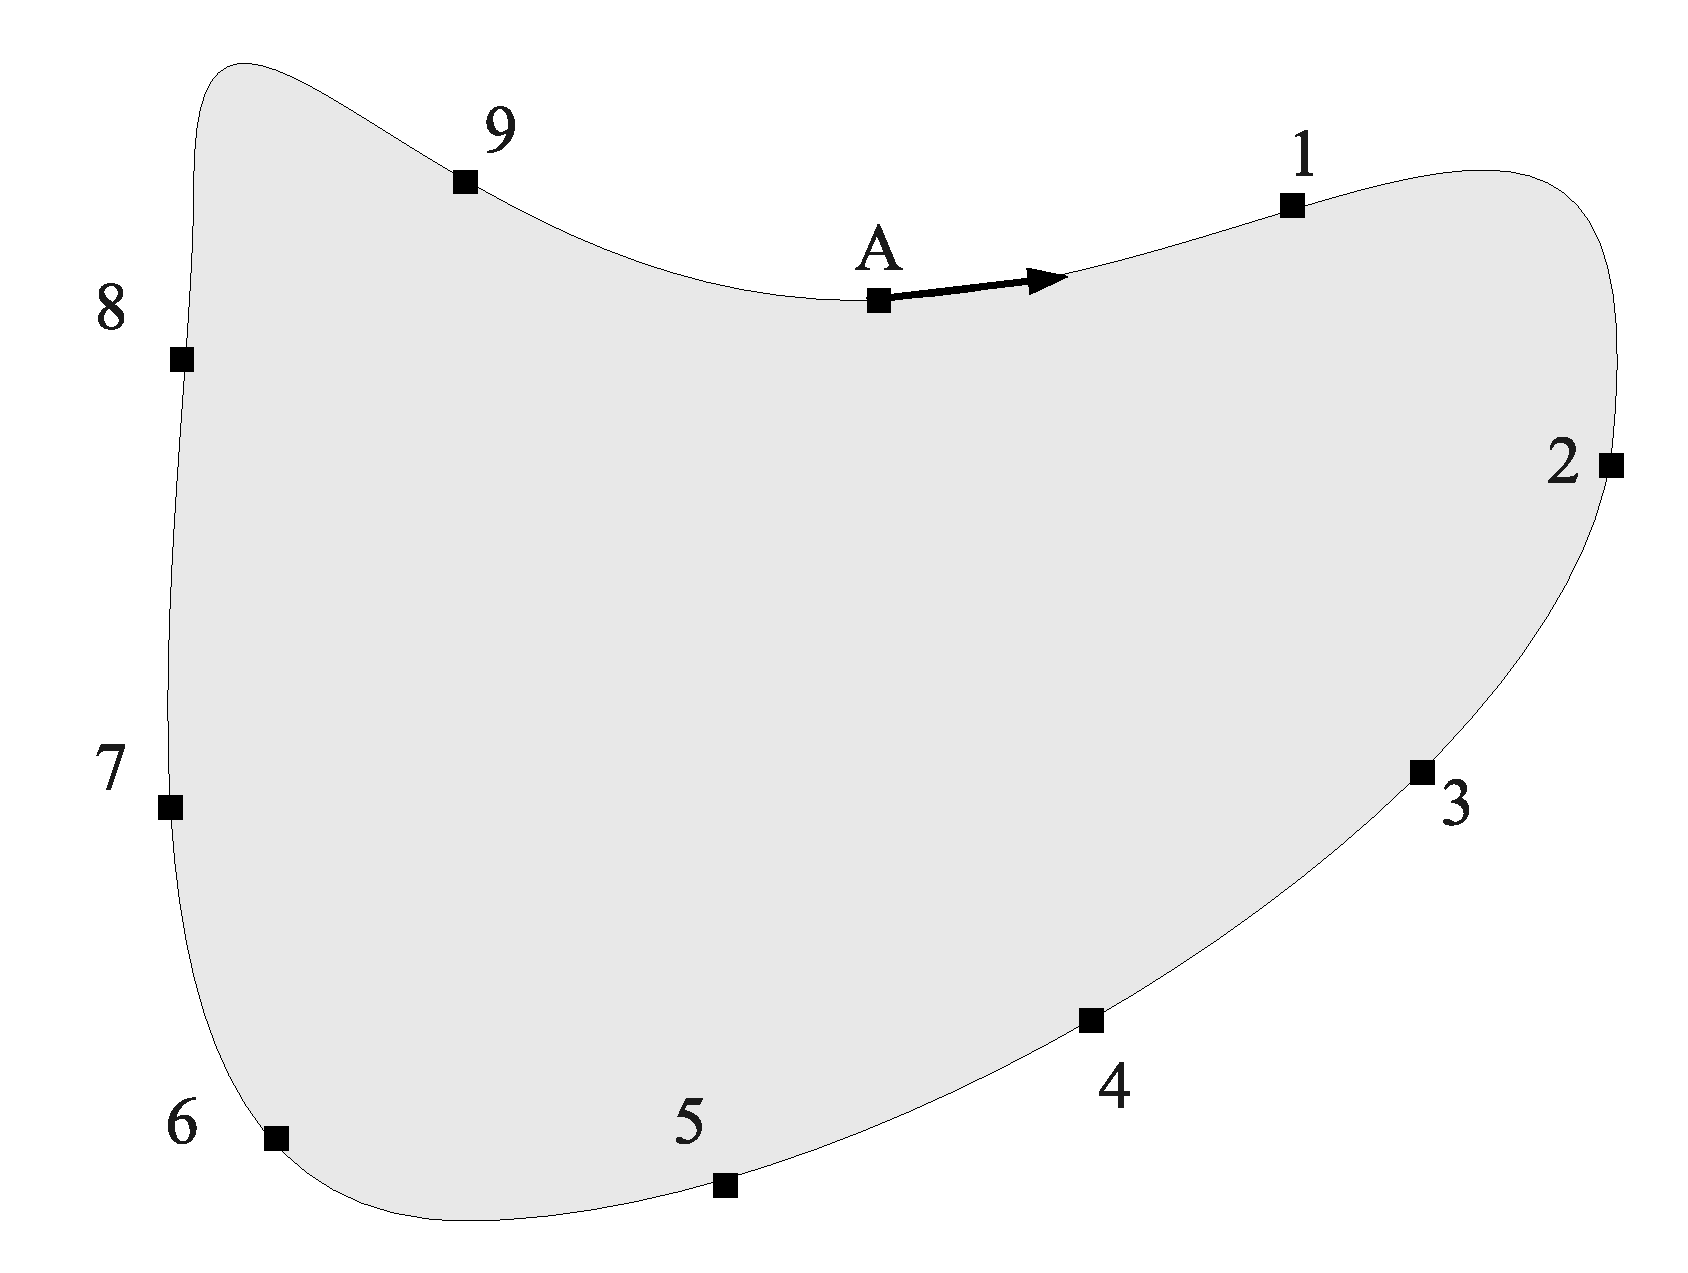
\includegraphics[width=0.5\textwidth]{./pista}
    \end{center}
\end{figure}

\newpage

Observa la l\'inea que se muestra a continuaci\'on. En el extremo izquierdo
coloca el n\'umero 4. En el extremo derecho coloca el n\'umero 8. Ubica en la
misma recta los siguientes n\'umeros:  \hfill \textbf{5 aciertos}

\textbf{a)}\,4.5 \hfill \textbf{b)}\,$4\displaystyle\frac{3}{4}$ \hfill
\textbf{c)}\,$\displaystyle\frac{22}{3} $ \hfill \textbf{d)}\,7.5 \hfill
\textbf{e)}\,6

\vspace{1.5cm}

\begin{center}
\line(1,0){350}
\end{center}

\vspace{1.5cm}

\section{Problemas}
Resuelve los problemas que se plantean a continuaci\'on.

\vspace{5mm}

Observa las figuras que se muestran a continuaci\'on y responde las preguntas.
\hfill \textbf{3 aciertos}

\begin{figure}[h]
    \centering
    \includegraphics[width=0.17\linewidth]{figures004.png}
    \includegraphics[width=0.17\linewidth]{figures005.png}
    \includegraphics[width=0.17\linewidth]{figures006.png}\\
    1 \hspace{2.5cm} 2 \hspace{2.5cm} 3
\end{figure}

?`Cu\'antos elementos tiene cada figura?

\vspace{1cm}

?`Cu\'antos elementos tendr\'a la siguiente figura?

\vspace{1cm}

?`Cu\'antos puntos habr\'a en la s\'eptima figura?

\vspace{1cm}

\vspace{1cm}

En una fiesta se repartieron $\frac{3}{4}$ de la gelatina entre los asistentes.
?`Cu\'al de las siguientes opciones expresa dos n\'umeros equivalentes a esa
fracci\'on? Explica tu procedimiento y marca la respuesta correcta.  \hfill \textbf{1 aciertos}

\begin{multicols}{2}

\begin{equation} \text{(A) \vspace{4mm}} \frac{750}{100} \text{\vspace{20cm} y
\vspace{20cm}} 7.500 \nonumber \end{equation}

\begin{equation} \text{(B) \vspace{4mm}} \frac{.75}{100} \text{\vspace{20cm} y
\vspace{20cm}} 0.0075  \nonumber \end{equation}

\begin{equation} \text{(C) \vspace{4mm}} \frac{7.5}{100} \text{\vspace{20cm} y
\vspace{20cm}} 0.075 \nonumber \end{equation}

\begin{equation} \text{(D) \vspace{4mm}} \frac{75}{100} \text{\vspace{20cm} y
\vspace{20cm}} 0.750 \nonumber \end{equation}

\end{multicols}

\vspace{5mm}


\end{document}
